\section{Il progetto OpenLDAT}
\subsection{Storia del progetto}
L'idea del progetto OpenLDAT nasce intorno a Marzo 2019, quando durante una presentazione di Google Stadia, discutendo i problemi di latenza dell'idea di eseguire videogiochi in streaming, viene mostrata al pubblico la tabella in figura \ref{fig:stadialies}.
\begin{figure}[h]
	\centering
	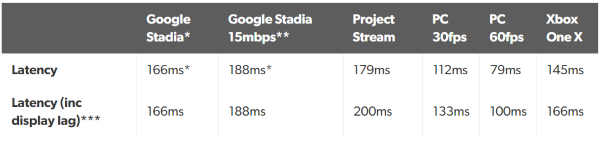
\includegraphics[width=\textwidth]{Chapter01/res/lies.png}
	\caption{Latenze secondo Google}
	\label{fig:stadialies}
\end{figure}

Ignorando per un momento il fatto che, secondo Google, Stadia ha lo stesso ritardo di input indipendentemente dal display utilizzato, che è impossibile, i numeri mostrati attirano subito l'attenzione di qualsiasi giocatore esperto, soprattutto su PC, poiché sembrano alquanto elevati. Sebbene sia vero che alcuni giochi, soprattutto quelli basati sulla storia che non richiedono di eseguire azioni rapide, hanno un ritardo elevato per migliorare la consistenza dei tempi dei fotogrammi, non è sicuramente rappresentativo nè del caso medio, nè del caso in cui la latenza è critica, come nei giochi musicali.

Vedendo questi dati, è stato deciso di costruire un semplice dispositivo per verificarli. Il dispositivo creato utilizzava un microcontroller per simulare la pressione di un tasto, la quale veniva ricevuta da un'applicazione OpenGL che generava un flash sullo schermo, che veniva rilevato da un fotoresistore collegato al microcontroller, il quale poi inviava via seriale il tempo trascorso tra l'invio del segnale e la ricezione del flash. La procedura veniva ripetuta 10 volte per avere un valore medio più accurato.

Eseguendo il test era stato ottenuto un ritardo medio di circa 50ms\cite{fdossena1}, su un display non "da gaming". Questo è rappresentativo del ritardo che subirebbe un videogioco programmato per avere una buona latenza sulla configurazione su cui era stato testato. Successivi test con un display a bassa latenza hanno abbassato la misura a circa 20ms.

Questa prima versione del progetto non è mai stata rilasciata per via di alcune limitazioni:
\begin{itemize}
	\item Il sensore utilizzato (un semplice fotoresistore) è relativamente lento\cite{adafruit_photores}, con un tempo di risposta di diversi millisecondi sia in salita che in discesa, il che significa che, senza un'accurata calibrazione, i risultati potrebbero essere seriamente sovrastimati
	\item Non c'era modo di regolare la soglia di attivazione del sensore se non variando delle resistenze (il sensore generava un interrupt)
	\item Il software non era in grado di gestire alcun tipo di disturbo nel segnale in arrivo dal sensore, il che causava risultati totalmente errati se veniva usato su display con retroilluminazione PWM, o dei vecchi CRT
	\item Il test funzionava solo in presenza dei flash sullo schermo, quindi non era possibile testare le diverse latenze di diverse applicazioni con questo metodo
\end{itemize}

A Novembre 2019, il lancio di Google Stadia ha attirato l'attenzione dei giornalisti del settore, i quali hanno cercato di eseguire un esperimento simile\cite{gamersnexus_stadia} \cite{gamersnexus_stadia2}, utilizzando un mouse modificato per accendere un LED quando viene premuto un tasto, e una telecamera ad alta velocità per misurare (con una risoluzione di qualche millisecondo) il tempo trascorso tra l'accensione del LED e l'inizio dell'azione sul display. L'utilizzo di metodi così "crudi" e manuali, anche da parte della stampa più tecnica e professionista evidenzia l'assenza di dispositivi per una facile analisi delle metriche di latenza dei display. Circa 2 anni dopo il lancio di Stadia, Google ha effettivamente raggiunto alcuni dei numeri promessi nella presentazione di Marzo 2019, ma al lancio l'opinione generale è stata pessima.

A Settembre 2020, Nvidia ha inviato un prototipo di un dispositivo chiamato Nvidia LDAT (Latency Display Analysis Tool) a diversi giornalisti del settore\cite{gamersnexus_nvidialdat}, un dispositivo quasi del tutto analogo a quello descritto in precedenza, ma con un sensore e un software migliori. Vedere questo progetto in azione ha fornito lo stimolo a far ripartire il progetto, che è poi stato realizzato nei mesi successivi. Sfortunatamente Nvidia ha deciso di non commercializzare il dispositivo, per cui si conosce poco dei dettagli sul funzionamento, ma verrà comunque discusso nel capitolo successivo sullo stato dell'arte.

Nel periodo tra Dicembre 2020 e Marzo 2021 è stato svolto gran parte del lavoro sul progetto OpenLDAT che, assieme ai dati sperimentali, è oggetto di questa tesi.

Nel periodo tra Marzo 2021 e Giugno 2021 è stata scritta questa tesi, sono stati eseguiti test su vari tipi di display, e sono state fatte migliorie agli algoritmi per assicurarne il buon funzionamento sul maggior numero possibile di display.

\subsection{Obiettivi del progetto}
Il progetto OpenLDAT si pone i seguenti obiettivi principali:
\begin{itemize}
	\item Fornire agli utenti un dispositivo per poter misurare, sia automaticamente che interattivamente, la latenza totale del proprio sistema, nel modo più accurato possibile, e permettendo il confronto tra sistemi e scenari diversi
	\item Rendere il dispositivo utilizzabile sul maggior numero possibile di display, anche in presenza forti disturbi come una retroilluminazione PWM
	\item Utilizzare il sensore nel dispositivo per fornire ulteriori metriche che non riguardano esclusivamente la latenza, ma anche la qualità del display, come una stima dei tempi di risposta reali dei pixel in diversi scenari
	\item Rendere il dispositivo facilmente costriuibile, utilizzando componenti off-the-shelf, facilmente reperibili, dai costi contenuti, e un software che non richieda calibrazioni
	\item Distribuire tutte le schematiche del dispositivo e il software su licenza libera, per consentire agli utenti di capirne il funzionamento e potenzialmente anche di apportare migliorie
\end{itemize}

Inizialmente, il progetto è rivolto principalmente a un pubblico tecnico, poiché è necessario sapersi assemblare il dispositivo da sè; qualora ci fosse interesse sufficiente per il progetto, però, diventerebbe possibile distribuirlo come prodotto finito e pronto all'uso; in questo caso il target si espanderebbe notevolmente, e diventerebbe usufruibile anche a un pubblico di giornalisti di tecnologia se non addirittura potenziali acquirenti in cerca di un nuovo monitor.

\subsection{Struttura del repository del progetto}
Tutti i file relativi al progetto OpenLDAT sono disponibili sul relativo repository GitHub\footnote{\href{https://github.com/adolfintel/OpenLDAT}{https://github.com/adolfintel/OpenLDAT}}. %è privato fino a fine tesi

Il respository è strutturato in questo modo:\begin{itemize}
	\item \texttt{App}: contiene il codice dell'applicazione OpenLDAT per PC e i file necessari per creare i package distribuibili. \begin{itemize}
		\item \texttt{OpenLDAT}: progetto dell'applicazione per NetBeans
		\item \texttt{Packaging stuff}: file necessari per creare i package distribuibili per Windows, GNU/Linux e MacOS
	\end{itemize}
	\item \texttt{Device}: contiene tutti i file relativi al dispositivo fisico OpenLDAT: \begin{itemize}
		\item \texttt{Case}: modelli 3D per il case stampabile e relative istruzioni
		\item \texttt{Firmware}: file relativi al firmware del dispositivo \begin{itemize}
			\item \texttt{OpenLDAT}: progetto del firmware per Arduino IDE
			\item \texttt{boards.txt}: dichiarazione del dispositivo per Arduino IDE
			\item \texttt{Libraries.zip}: copia di backup delle librerie necessarie per compilare il firmware, qualora non fossero più disponibili in futuro
			\item \texttt{Prebuilt}: firmware precompilato per flashare il dispositivo senza Arduino IDE
		\end{itemize}
		\item \texttt{Hardware}: file relativi al circuito del dispositivo: \begin{itemize}
			\item \texttt{OpenLDAT\_Model1.fzz}: progetto del dispositivo per Fritzing
			\item \texttt{gerber}: file del PCB del dispositivo in formato standard gerber per la stampa
		\end{itemize}
	\end{itemize}
	\item \texttt{Docs}: documentazione del dispositivo e dell'applicazione, in inglese
\end{itemize}

Questo conclude il capitolo introduttivo. Nei capitoli successivi verrà discusso lo stato dell'arte, confrontando OpenLDAT con progetti, dopodiché verrà introdotto il dispositivo stesso.
